\documentclass[letterpaper, paper,11pt]{AAS}

\usepackage{bm}
\usepackage{amsmath}
\usepackage{subfigure}
\usepackage[colorlinks=true, pdfstartview=FitV, linkcolor=black, citecolor= black, urlcolor= black]{hyperref}
\usepackage{overcite}
\usepackage{footnpag}
\usepackage{tikz}
\usepackage{float}
\usepackage{comment}
\usepackage{booktabs}
\usetikzlibrary{shapes.geometric, arrows.meta, positioning}
\tikzstyle{process} = [rectangle, minimum width=3.5cm, minimum height=1cm, text centered, draw=black, fill=blue!10]
\tikzstyle{decision} = [diamond, minimum width=3cm, minimum height=1cm, text centered, draw=black, fill=yellow!20]
\tikzstyle{startstop} = [ellipse, minimum width=3cm, text centered, draw=black, fill=red!20]
\tikzstyle{arrow} = [thick, ->, >=stealth]
\PaperNumber{25-787}

\begin{document}

\title{Advanced Modeling Techniques for Analyzing Space Debris Fragmentation and Evolution}

\author{Juan F Puerta-Ibarra\thanks{Professor, Department of Mechanical and Aerospace Engineering, Universidad de Antioquia, calle 67 No. 53 - 108, Medellín - Colombia},  
Bonnie Prado Pino\thanks{Adjunct Professor, Department of Mechanical and Aerospace Engineering, Universidad de Antioquia, calle 67 No. 53 - 108, Medellín - Colombia. Design Engineer, Odyssey Space Research, Houston, TX 77058},
\ and Nicolas Muñoz-Galeano \thanks{Professor, Research Group in Efficient Energy Management (GIMEL), Department of Electrical Engineering, Universidad de Antioquia, calle 67 No. 53 - 108, Medellín - Colombia}
}

\maketitle

\begin{abstract}

The increasing presence of space debris poses significant challenges to orbital sustainability, necessitating advanced modeling techniques for long-term analysis. This research presents a validated computational framework for analyzing the evolution of debris in high-density orbital environments, incorporating geopotential perturbations. The framework enables forward propagation utilizing N-body symplectic integrators from the REBOUND package, facilitating a comprehensive assessment of collision risks and debris evolution. This study validates the framework's accuracy, performance, and long-term stability against high-fidelity tools using a large-scale simulation of 20,000 objects in Low Earth Orbit (LEO). Results demonstrate excellent positional agreement (sub-kilometer deviation over 24 hours), significant computational scalability (propagating thousands of fragments orders of magnitude faster than traditional tools), and superior long-term energy conservation. This approach enhances the fidelity of orbital debris models and informs mitigation strategies for sustainable space operations.
\end{abstract}

\section{Introduction}
Fragmentation of space debris is a critical issue in the context of increasing space activities and the sustainability of the orbital environment. Since the dawn of the space age, the number of artificial objects in orbit has grown significantly. As of 2023, estimates indicate over 35,000 tracked objects larger than 10 cm in diameter, with a far greater number of smaller, untrackable but still dangerous fragments\cite{european_space_agency_space_nodate}. This growth is being accelerated by the "NewSpace" era, characterized by the deployment of large satellite constellations for global internet and Earth observation, which drastically increases the density of operational objects in key orbital regimes, particularly Low Earth Orbit (LEO).

Fragmentation events, which occur due to collisions, explosions, or structural failures, are the primary contributors to the debris population. A particular concern is the \textit{Kessler syndrome}, a scenario first proposed by Donald Kessler in 1978, in which the density of objects in LEO becomes so high that collisions between objects cause a cascade effect, creating more debris and exponentially increasing the likelihood of further collisions\cite{kessler_collision_1978}. If triggered, this self-sustaining chain reaction could render certain orbits unusable for generations.

The intentional destruction of satellites, such as the 2007 Chinese anti-satellite (ASAT) test, and accidental fragmentation events, like the landmark 2009 collision between the active Iridium 33 and defunct Cosmos 2251 satellites, have already contributed significantly to the current debris population. Such catastrophic events can create thousands of new, long-lived fragments\cite{wang_analysis_2010}. The dynamics of space debris fragmentation are complex, influenced by the physical properties of the objects, the nature of the event, and the intricate orbital environment. This underscores the urgent need for high-fidelity modeling techniques to accurately predict the evolution of the debris environment and ensure the long-term viability of space operations.

\section{Background on Debris Fragmentation}

Understanding the causes of space debris fragmentation is crucial for accurate modeling. The primary sources of fragmentation are collisions, explosions, and deliberate actions.

\subsection{Fundamentals of Space Debris}

Space debris encompasses defunct satellites, spent rocket stages, fragments from collisions, and other remnants of human space activities. It populates Earth's orbit, posing challenges to operational spacecraft and future space missions. Understanding the dynamics of space debris involves considering its types and the mechanisms leading to its creation. Space debris can be broadly categorized into two main types: large objects and small particles. Large objects include defunct satellites, spent rocket stages, and fragments from previous collisions. Small particles, often referred to as micrometeoroids or paint flecks, result from the continual erosion and fragmentation of larger objects due to natural forces in the space environment, orbital perturbations, and the upper atmosphere, among others.

As the quantity of artificial satellites and objects orbiting the Earth continues to rise, as shown in Figure~\ref{fig:typeobject}, the likelihood of collisions among these satellites also escalates. These collisions would result in the creation of orbiting fragments, each contributing to an increased probability of subsequent collisions. This sequence of events could lead to the expansion of a debris belt encircling Earth, drawing parallels with theories regarding the formation of asteroid belts. The flux of debris in such an Earth-orbiting belt might surpass the natural influx of meteoroids, thereby influencing the design considerations for future spacecraft. Using a mathematical model, predictions were made regarding the potential rate of formation for such a belt. Under specific circumstances, the initiation of this belt could commence within the current century and pose a notable challenge in the subsequent century. The presence of numerous undetected fragments resulting from spacecraft explosions could
potentially shorten this time frame. However, the early adoption of specialized launch restrictions and operational protocols has the potential to substantially postpone the formation of the debris belt.

\begin{figure}[!htb]
    \centering
    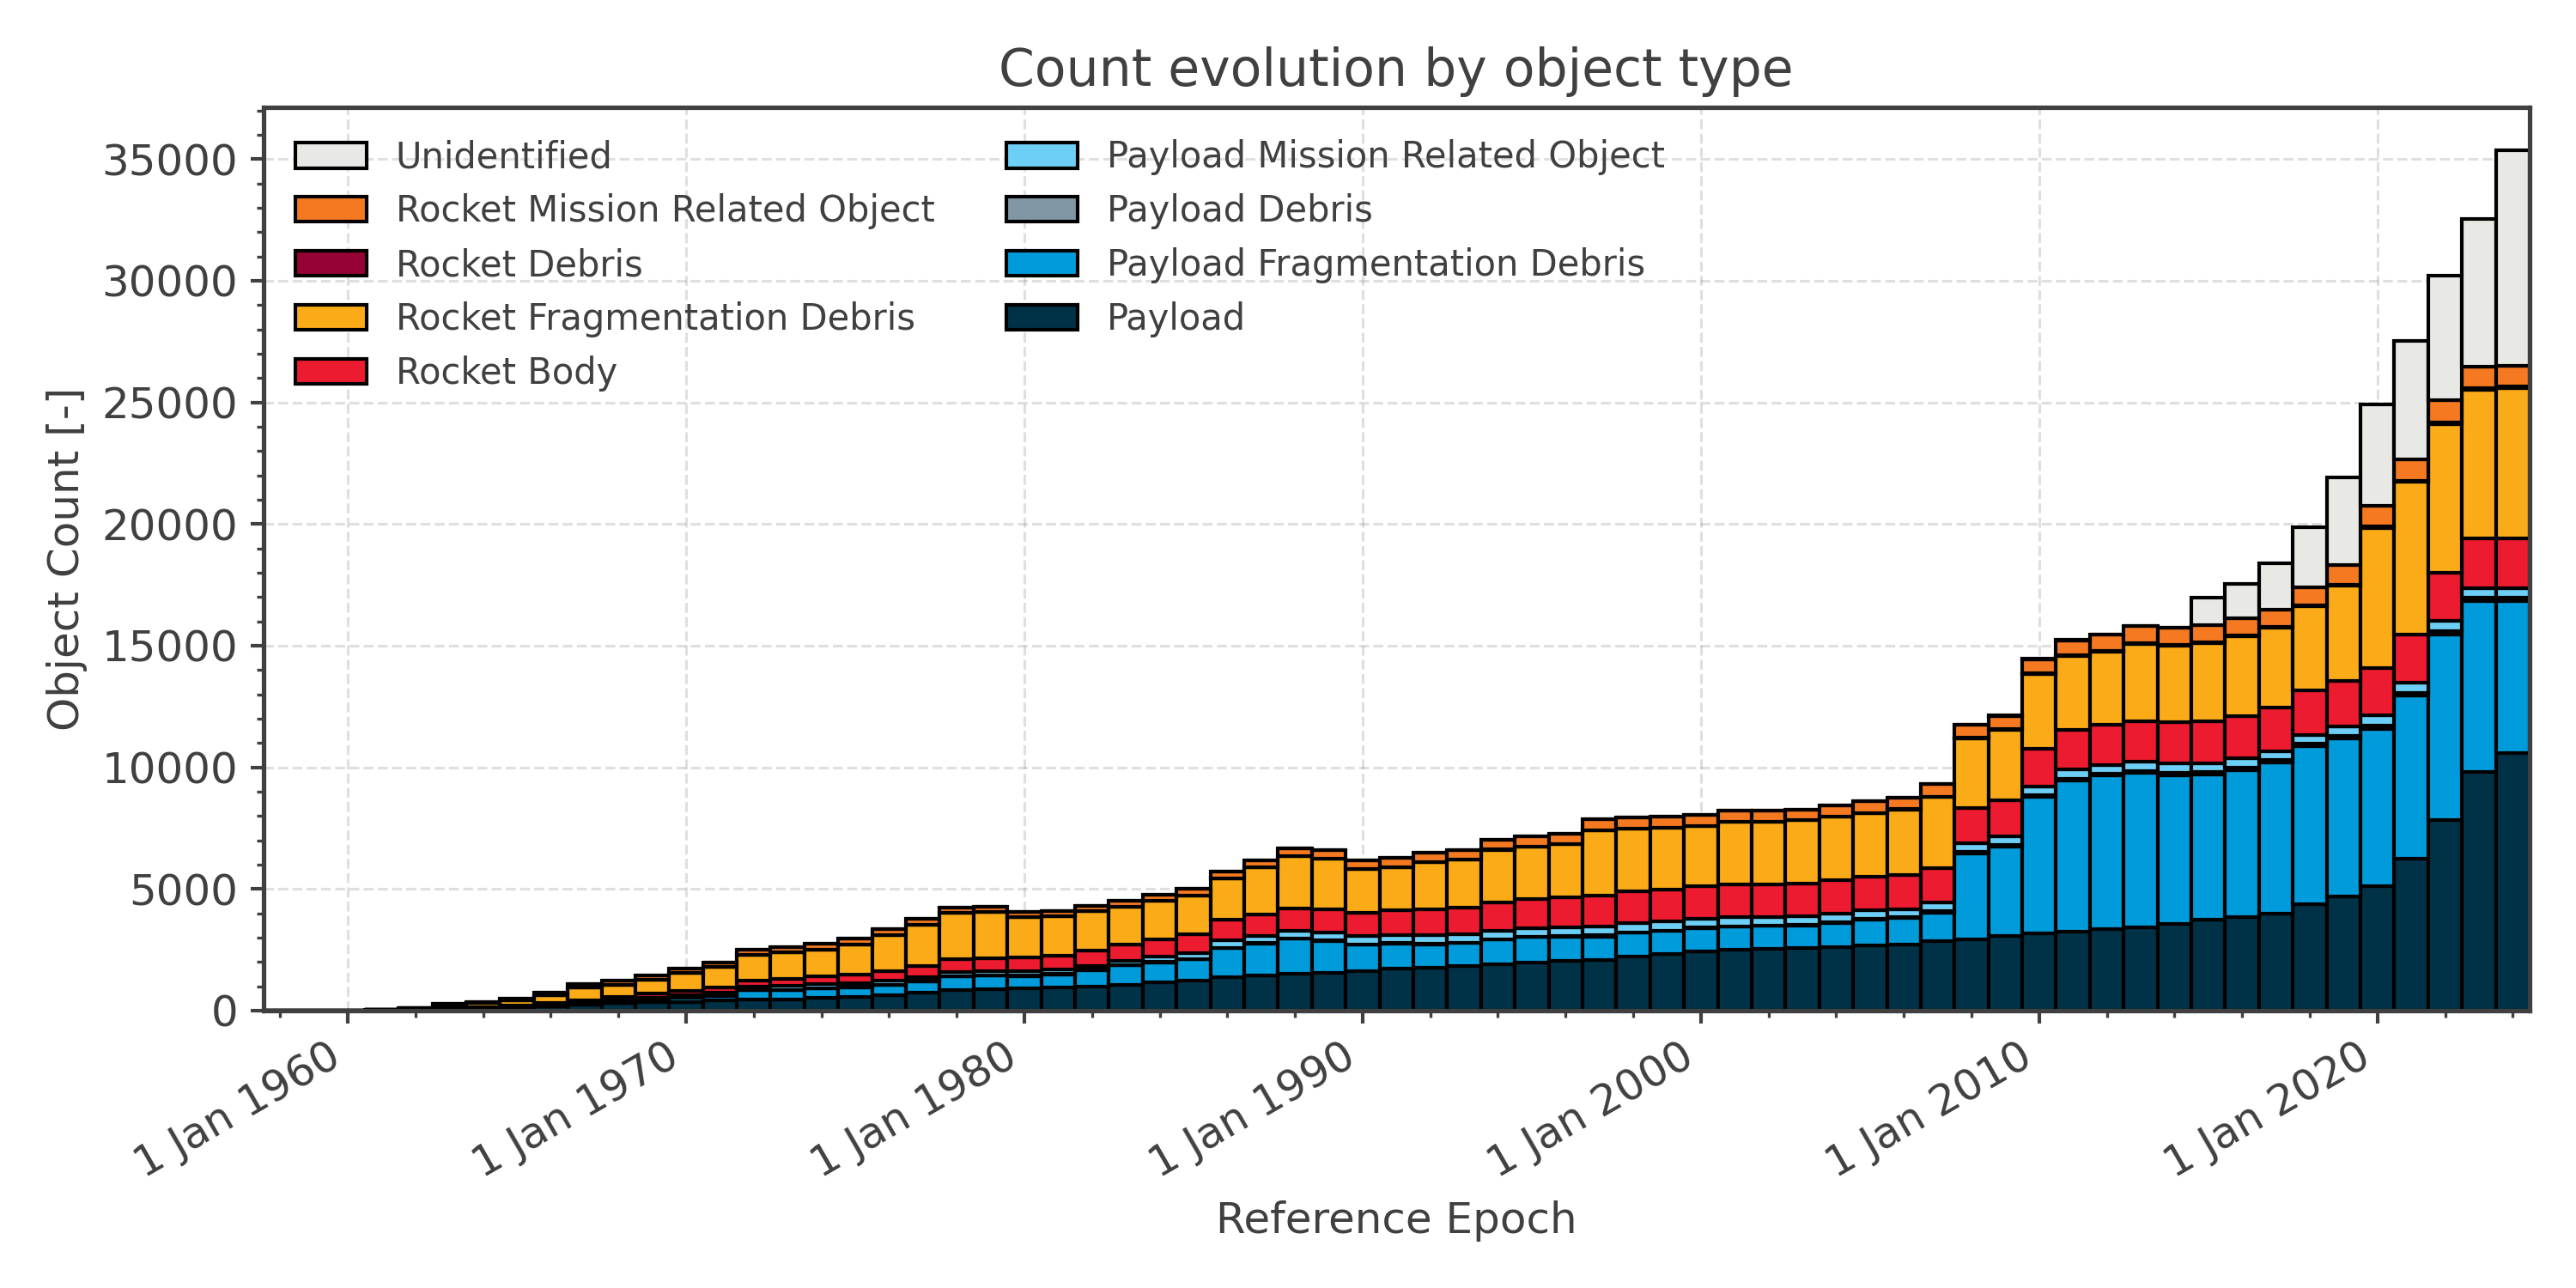
\includegraphics[width=\linewidth]{allEvoTypeCnt.png}
    \caption{Evolution of the number of objects in geocentric orbit by object class. Source: \href{https://sdup.esoc.esa.int/discosweb/statistics/}{Space Debris Environment Report issued by ESA's Space Debris Office, 2023}}
    \label{fig:typeobject}
\end{figure}

The concept known as the Kessler syndrome, initially theorized by Don Kessler and Burt Cour-Palais in 1978, has been a focal point in extensive global research. This syndrome, which revolves around the collision among space objects, is considered one of the most challenging aspects of managing orbital debris~\cite{kessler_collision_1978}. It has the potential to generate a substantial number of fragments per collision event, posing a significant threat. If the frequency of collisions surpasses the natural atmospheric cleansing process, a chain reaction may ensue, gradually but inevitably increasing the overall debris population in densely populated areas of space. This phenomenon has garnered widespread attention, leading to numerous publications, dedicated workshops, and special sessions during international congresses. Recent studies, focusing primarily on major fragmentations in 2007 and 2009, suggest that the Kessler syndrome has indeed been set in motion. The consensus emerging from these studies
underscores the importance of adhering to internationally agreed-upon mitigation rules to sustain space activities in the long term. Active deorbiting measures, specifically targeting at least five large objects annually from the most densely populated orbital regions, are deemed necessary for effective mitigation and remediation efforts. Collective findings emphasize the imperative to implement strategies to preserve the sustainability of long-term space operations.~\cite{bonnal_active_2013}

Spacecraft fragmentation is a complex dynamic problem involving collisions, explosions, and gravitational interactions, and space weather must be included to characterize the problem correctly, due to the extreme operational conditions and mission design requirements. Researchers model the fragmentation process, in the first stage, using numerical integration techniques~\cite{isoletta_orbital_2021}, such as Runge-Kutta or Prince-Dormand, e.g., to obtain the state vector (position and velocity of space objects) or their orbital elements (semi-major axis, eccentricity, inclination, etc.) and then propagating its positional state in backward or forward direction, depending on the ephemerides of the event. One initial idea is to get the latest state vector (position and velocity coordinates in the Cartesian coordinate system) with their TLE (Two Line Elements) information, simulate it going backward, and find how the particles were ejected after the fragmentation event. Using computational analysis, such as orbital
propagators based on physics dynamics, is the first step to understanding the equations and models ruling the phenomena. More advanced models are required since they involve not only the motion of the objects in space but also the fragmentation process in orbit.

\section{Conjunction of Objects in Space}

In the past decade, a combination of economic incentives and political objectives has accelerated space launches, contributing to a continuous growth in both active satellites and space debris. Consequently, satellite operators and space agencies globally have a keen interest in precisely assessing the risk of potential collisions and determining necessary collision avoidance maneuvers. Recognizing that unmitigated collision risks in the short term can lead to long-term environmental degradation, proactive measures are imperative.

As universally recognized within the Space Situational Awareness community, the frequency of conjunctions is anticipated to significantly increase in the future, primarily due to the proliferation of new megaconstellations, small satellites, and other payloads. The introduction of these novel payloads is expected to exert a considerable impact on the space environment, manifesting in heightened collision risks, atmospheric pollution, and surface impacts. The increasing number of operational satellites accentuates the relevance of collision avoidance strategies, particularly in scenarios involving two active satellites. In such cases, the assessment of conjunctions and maneuvers necessitates a distinct approach compared to situations involving an active satellite and space debris, where only the active satellite is capable of executing maneuvers.~\cite{oltrogge_collision_2016}

\section{Space Debris Fragmentation}

Since 1961, more than 80 incidents of satellite fragmentation have been identified. These events account for one-third of all human-made objects in space documented since the launch of Sputnik 1 and constitute half of the satellites currently orbiting Earth. The two recognized causes of artificial satellite break-ups are accidental occurrences, often related to propulsion malfunctions, and deliberate actions, such as military-related onboard explosions. However, the reasons behind fifty percent of satellite breakdowns remain unknown, although in Figure~\ref{fig:enter-label} the unknown causes are more likely to be predominant. The continual growth in the population of near-Earth space debris raises valid concerns regarding the increasing likelihood of collisions between satellites. The constraints of ground-based radars imply that the actual number of Earth-orbiting satellites could be significantly higher than officially registered. Recent laboratory experiments indicate that a substantial
number of potentially hazardous fragments could be released during hyper-velocity collisions in space.~\cite{johnson_history_1985}

The effects of spacecraft fragmentation on space sustainability can be analyzed using various metrics, such as the creation of new debris, the risk of collision with operational spacecraft, and the potential impact on-scientific observations. Mitigation of space debris can be achieved through various methods, such as active debris removal and collision avoidance techniques. The effectiveness of these methods can be assessed through more precise numerical simulations and statistical analyses.

\begin{figure}[!htb]
    \centering
    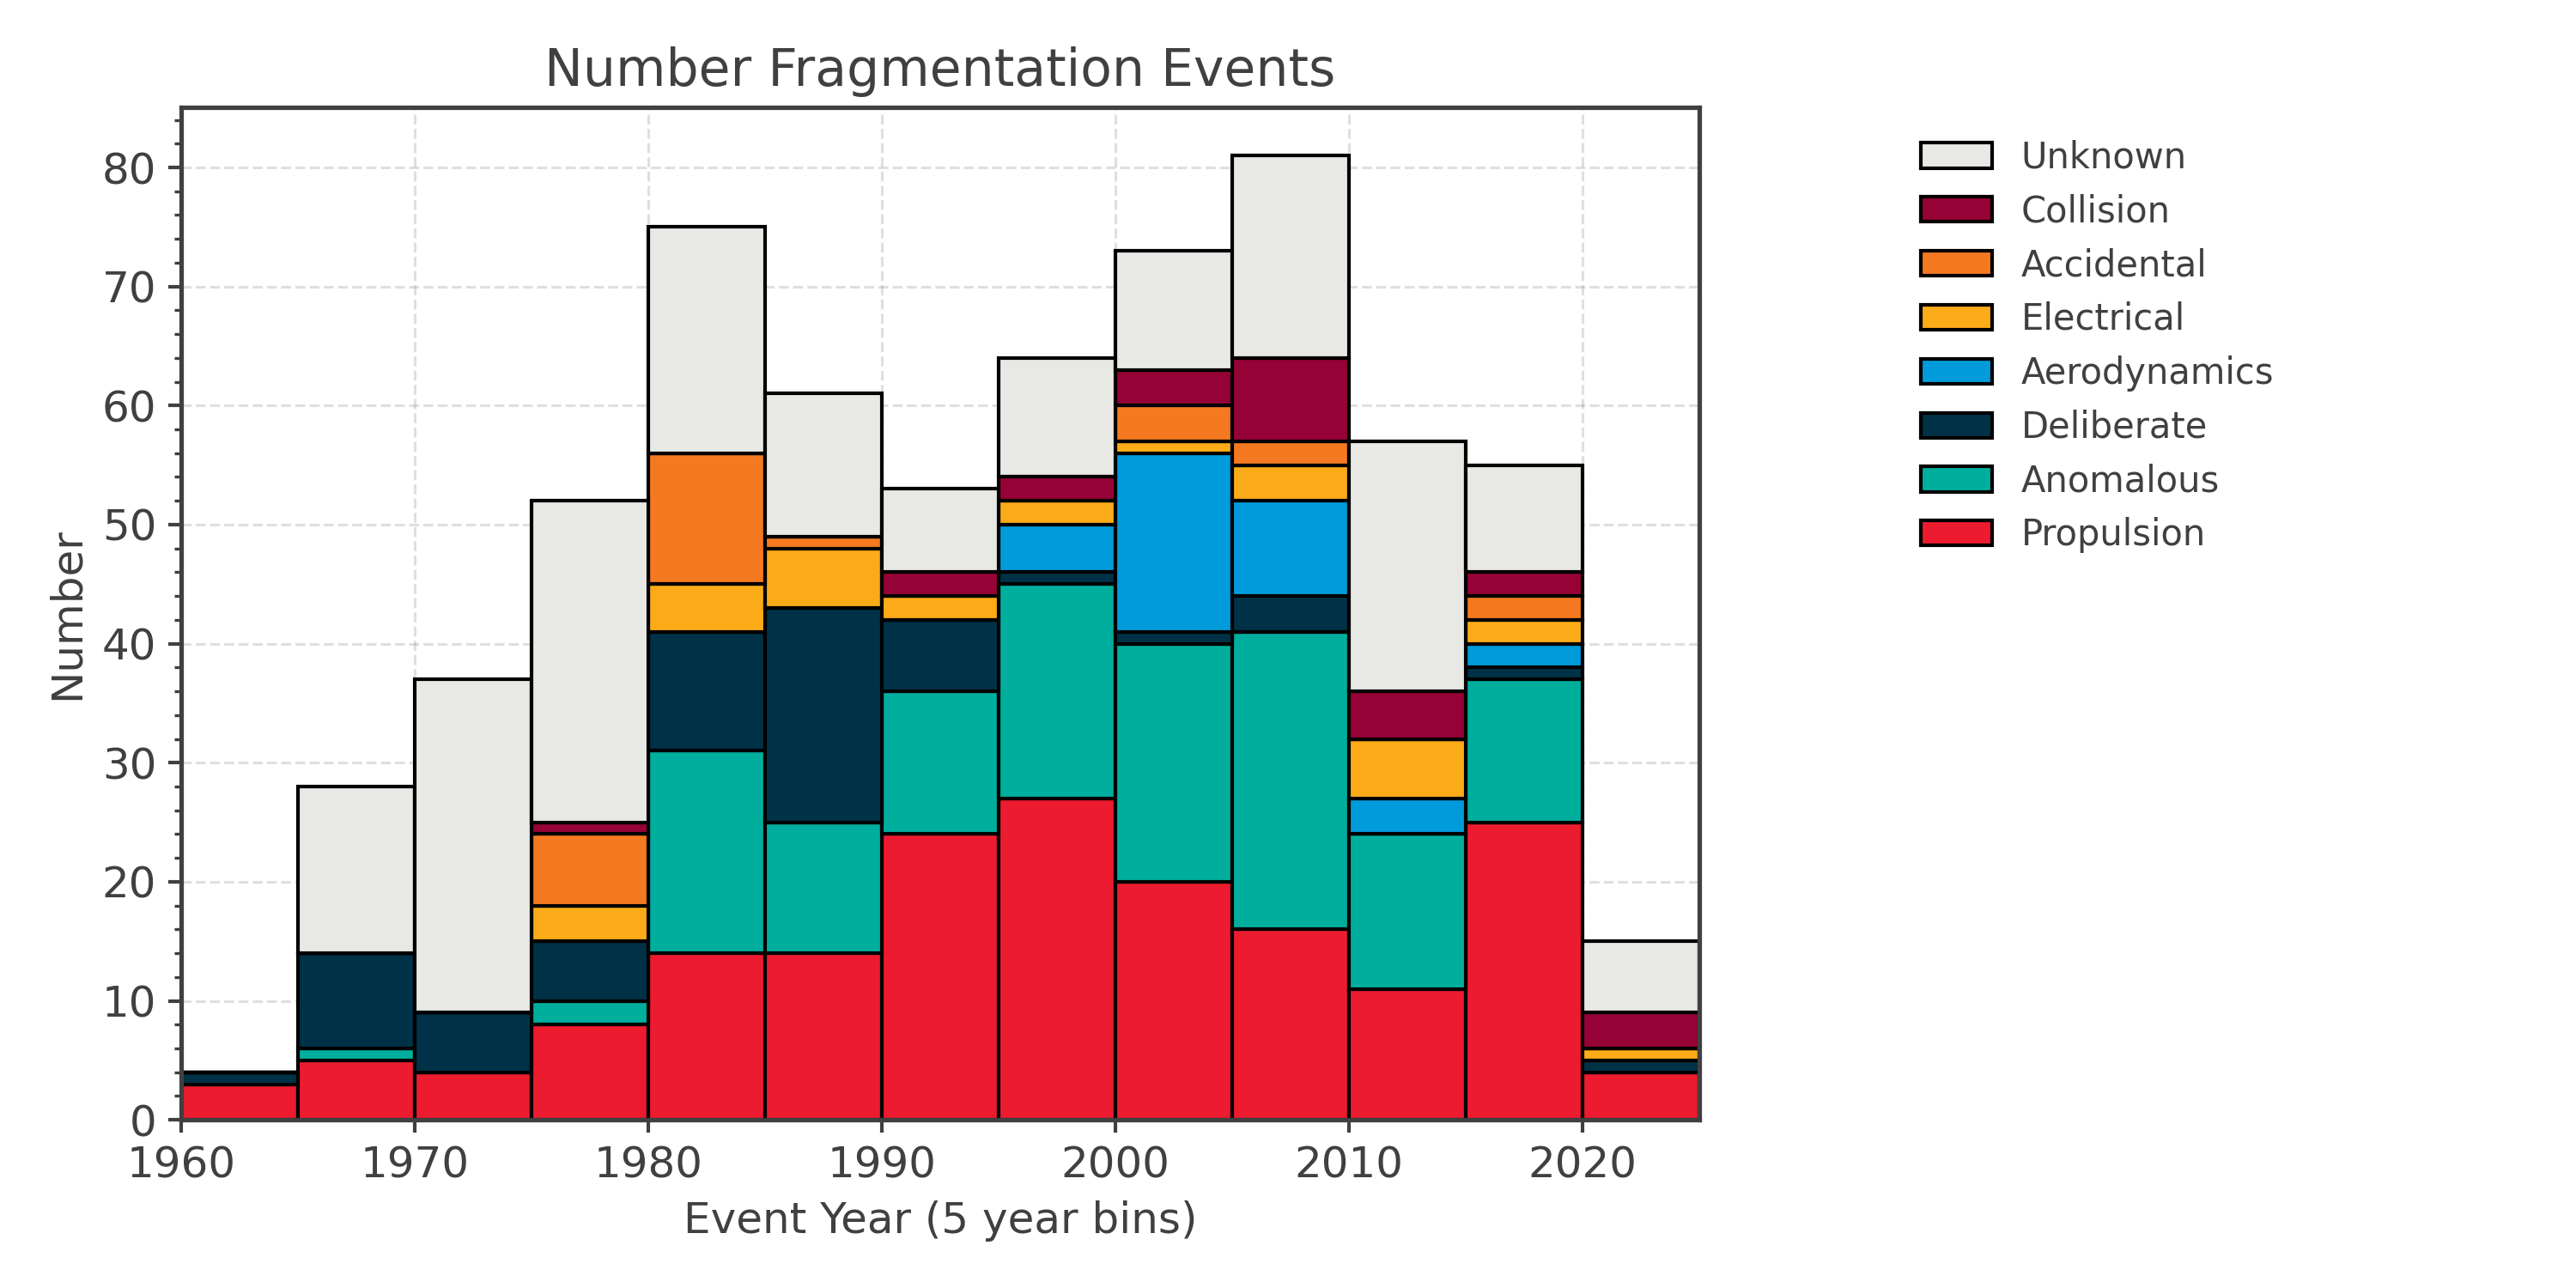
\includegraphics[width=\linewidth]{eventCausesPerEY_abs.png}
    \caption{Historical trend of fragmentation events per event cause. The last bin covers until the year 2022. Source: \href{https://sdup.esoc.esa.int/discosweb/statistics/}{Space Debris Environment Report issued by ESA's Space Debris Office, 2023}}
    \label{fig:enter-label}
\end{figure}

\subsection{Causes of Space Debris Fragmentation}

Understanding the causes and effects of space debris fragmentation is extremely important to determine the behavior, modeling, and development of new approaches and computational tools for appropriate analysis. Furthermore, understanding these factors is crucial to modeling events more precisely and devising futuristic scenarios based on the initial data. Several primary factors contribute to the fragmentation of space debris.

On average, there have been 11.2 instances of non-deliberate fragmentations annually in the space environment over the past two decades. While this figure remains relatively consistent, the impact of each event varies. When considering the lifespan of the generated fragments, this number notably decreases to 2.5 per year, and further drops to 0.4 per year when systematic and unexplained events are excluded from the analysis. This suggests that non-collisional events, which can have a substantial environmental impact, persist, potentially attributed to the reuse of a design with known issues. In particular, fragmentations other than collisions currently represent the primary source of space debris. The escalating launch traffic and the enduring nature of space debris events in the low Earth orbit contribute to a considerable conjunction risk in the most congested Earth orbits.~\cite{european_space_agency_space_nodate}

\subsubsection{Collisions}
High-velocity impacts between space debris and operational satellites or other assets in orbit occur at high relative velocities, generating smaller fragments in the process with a large amount of energy released. These collisions have been studied, and their implications are documented, but the amount of information is still not enough for a more profound analysis.

Cascading collisions can result from these initial collisions, leading to further break-up events and exacerbating the debris problem. The cascade effect is a significant concern in the context of space debris dynamics and mitigation efforts, based on the initial concept explained by Don Kessler in 1978. The primary idea behind this concept is that a single collision between two space objects can create a cloud of smaller debris fragments. These fragments, in turn, pose a significant risk to other operational satellites and space assets, potentially leading to additional collisions and more fragmentations.~\cite{kessler_environment_1985}

\subsubsection{Explosions}
Explosive decompression can occur due to explosions of defunct satellites, spent rocket stages, or malfunctioning components. These events can be due to various factors, including residual propellants, batteries, or other hazardous materials within the system, mostly after some years of operations in space. The outcome is often the disintegration of the original object into smaller fragments.

When an explosion event occurs, it can generate a cloud of smaller fragments. The sizes of these fragments can vary widely, ranging from large pieces to tiny shards and even micrometer-sized particles. The number of fragments created depends on the magnitude of the explosion, the materials involved, and the specific circumstances of the event. These fragments are then released into various orbits around the Earth.

Accurate modeling of space debris from explosion events is essential for space situational awareness and collision avoidance. As discussed above, mathematical models and simulations are used to predict the trajectories and behavior of these fragments. However, the sheer number of debris pieces and the complex dynamics of their orbits make this a challenging task.

\subsubsection{Natural Forces}
Space debris is subject to natural forces, including micro-meteoroid impacts. These impacts gradually erode and fragment objects over time, contributing to the overall fragmentation of space debris. The impact of natural forces is a critical aspect in understanding the long-term dynamics of space debris. Micrometeoroids, tiny particles present in space, can collide with space debris fragments, leading to surface erosion and potential fragmentation. These impacts can gradually degrade the structural integrity of debris objects, causing them to break into smaller pieces or generating cracks and fissures.

Orbital fragments, once released into the Earth's orbit, are subjected to various natural forces that contribute to their evolution and behavior over time. These natural forces, originating from the space environment itself, can impact the dynamics and characteristics of space debris, influencing their trajectories and potential collision risks. By being in orbit, gravitational interactions with additional celestial bodies besides Earth, such as the Moon or the Sun, can perturb the orbits of space debris fragments. These gravitational forces can cause variations in the orbital parameters of residual objects, leading to changes in their positions, velocities, and orbital planes. Over time, these perturbations can result in alterations to the distribution and density of debris fragments within different orbital regions.

Space weather, primarily created by the Sun, is an important factor to consider, since solar radiation exerts pressure on these objects, especially those with larger surface areas. This pressure can influence the orbits of debris objects, leading to changes in their trajectories over time. These forces, while relatively weak, can gradually alter the paths of debris fragments, potentially increasing the risk of collisions with other space assets. Moreover, the Earth's environment from the atmosphere creates drag, leading to a gradual decrease in their orbital altitudes. This drag force results from the interaction between elements in low-earth orbit and the Earth's atmosphere, causing their positions to decay over time. As their orbits decay, the debris fragments may re-enter the Earth's atmosphere, leading to their eventual incineration or impact on the planet's surface.

\subsubsection{Deliberate Actions}
Deliberate actions in space, such as anti-satellite (ASAT) tests, significantly contribute to space debris fragmentation. These actions involve the intentional destruction of a satellite or space object, often for military or scientific purposes. The primary reason for these activities leading to the fragmentation of space debris is the violent nature of the destruction, from a kinetic point of view, which generates a large number of debris fragments. Certain space missions intentionally fragment objects in orbit, often for scientific research or military purposes. 

The Fengyun-1C event from an ASAT (Anti-Satellite Weapons Test) made by China in 2007, is a notable example of the impact of the test in the space environment in LEO. These deliberate actions can lead to the generation of additional debris fragments, contributing to the already complex space debris environment.

 In an ASAT test, a satellite or space object is typically destroyed using a kinetic device, usually from a missile launched from the surface of the Earth or by a military aircraft. When the impact process is produced, it causes the target satellite to rapidly decompress. This explosive decompression results in the disintegration of the satellite into numerous smaller pieces. These fragments can vary in size and can include structural components, electronics, and other satellite materials. Fragments produced during an ASAT test are ejected from the site of the explosion at high relative velocities, often exceeding the speeds typical for space debris in orbit. These high velocities can increase the kinetic energy of the fragments, making them potentially more dangerous and more prone to damage in the event of a collision.~\cite{sorge_orbital_2008}

\section{Tracking and Cataloging}
Tracking and cataloging space debris objects is a challenging but vital task for space debris fragmentation analysis. The difficulty arises from the vast number of objects in orbit, their small sizes, varying orbits, and the need for continuous monitoring. However, the importance of this endeavor cannot be overstated, as it forms the foundation for understanding the behavior and risks associated with space debris.

Space is crowded with objects, including operational satellites, defunct spacecraft, spent rocket stages, and various fragments. Some of these objects are as small as paint chips, making them challenging to track. The task is further complicated by the diversity of orbits they occupy, from low Earth orbit (LEO) to geosynchronous orbit (GEO). Tracking space debris is akin to finding and monitoring thousands of moving targets in a vast, dynamic, and three-dimensional environment. Accurate tracking and cataloging are essential for
understanding the distribution of space debris in Earth's orbit. The data gathered through tracking systems helps identify regions with higher debris density and areas with a greater risk of collisions. This knowledge is critical for spacecraft operators to plan and execute maneuvers to avoid potential collisions.~\cite{watson_optical_2019}

The process of tracking debris in orbit enables the prediction of close approaches and potential collisions between those elements and operational satellites. Timely warnings of such events allow satellite operators to adjust orbits or take other preventive measures to protect their assets. This is crucial for maintaining the safety and functionality of operational satellites.~\cite{noauthor_space_nodate}

\section{Fragmentation Modeling}

Small objects in debris simulation models require a simplified but elegant and accurate approach to describe the evolution of a cloud of objects in space, making the analysis of a collision or explosive event a very demanding process. 

Analytical models~\cite{letizia_continuity_2014} describing the behavior of artifacts in orbit have been proposed mainly for small-duration events where the forces can be represented by Hamiltonian mechanics. The analysis of long-term population where space debris density is high was presented by McInnes in 1993, by considering the population in Low Earth Orbit as a fluid with continuous properties. This approach has been complemented by Nazarenko, who describes the progression of the number of objects in LEO based on the continuity equation with his own development~\cite{letizia_multidimensional_2016}:

\begin{equation}
\frac{\partial N_j}{\partial t}=-W_j\frac{\partial N_j}{\partial r}-N_j\frac{\partial W_j}{\partial r}+\dot{N_j} 
\end{equation}

where $N_j(r,t)$ is the number of elements in the $j^{th}$ bin regarding size, perigee altitude (rp), eccentricity (e), inclination (i), and ballistic coefficient. $W_j$ is the radial velocity of the objects, and $\dot{N_j}$ is the rate of variation in the number of objects based on external causes. Based on the equation presented, the discussion is about the advantage of having a statistical model based on density compared to a deterministic model whose results are obtained by inputs and a set of equations describing the system, without randomness or uncertainty.

To create a precise model for space debris, it is essential to not only account for recent occurrences but also maintain a comprehensive historical record of in-orbit fragmentations on an ongoing basis. Presently, there are 261 recognized fragmentation events, with each one treated as a distinct incident in the modeling process. While there are some additional events labeled as unknown anomalies, they are excluded from the fragmentation modeling phase. All the acknowledged events are classified as either explosions or (non-)catastrophic collisions, with detailed data on event characteristics such as mass and collision velocity. Of these 261 events, 247 are classified as explosions, making up approximately 95\% of the total. The remaining 14 events are designated as confirmed, for example, the Fengyun-1C Anti-Satellite Test, and assumed collisions. However, when examining the overall amount of tracked debris by the Space Surveillance Network (SSN), there are
twice as many fragments resulting from explosions compared to those from collisions. Figure~\ref{fig:breakupincident} shows the number of fragmentations over the last 60 years~\cite{horstmann_survey_2018}. 

\begin{figure}[!htb]
    \centering
    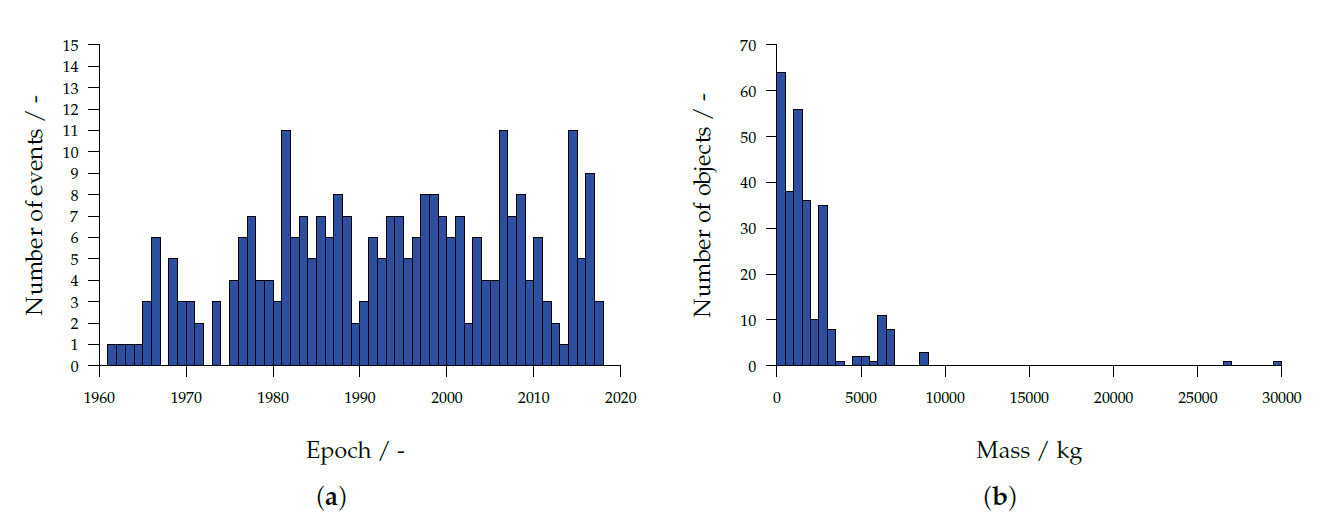
\includegraphics[width=\linewidth]{Fig1.png}
    \caption{Assessment of the historical record of breakup incidents, including (a) the yearly count of in-orbit breakups, and (b) statistical data in the form of a histogram regarding the distribution of objects per fragmentation mass.}
    \label{fig:breakupincident}
\end{figure}

The average annual count of fragmentations is 4.9 (with a standard deviation of 2.8), and there is no observable trend of decline or significant alteration. However, there was a slight reduction in fragmentations over three years following the implementation of the Inter-Agency Space Debris Coordination Committee (IADC) with its Space Debris Mitigation Guidelines in 2010. 
Figure~\ref{fig:breakupincident}(b) illustrates the examination of the fragmented mass over the years, highlighting that most of the objects that underwent fragmentation had a mass of less than 500 kg. On the opposite end of the spectrum in the histogram, there are two instances featuring a fragmentation mass of 26,000 kg and 30,000 kg. These occurrences date back to the late 1960s during the Apollo program; however, owing to their low orbital altitudes of below 300 km, nearly all fragments re-entered Earth's atmosphere, thereby making minimal long-term contributions to the space debris environment.

In recent times, the space sector has witnessed a notable phase of growth and transformation, characterized by the emergence of a burgeoning startup culture, often referred to as "NewSpace" or "the new space era". This shift is commonly linked to an amplified engagement of private investors and a change in priorities, diverging from the conventional practices of government and military-industrial entities. According to reports from Bryce Space and Technology, there has been a remarkable over twelve-fold rise in the annual average of investors in the space domain since the year 2000~\cite{diserens_newspace_2020}.

The phenomenon of fragmentation has been recognized as a critically significant aspect to focus on, and it's especially collisions that are anticipated to increasingly contribute to the generation of new space debris in the future setting. In the broader scope of creating models for the debris environment, understanding the mechanisms by which objects undergo fragmentation is vital. This comprehension not only helps in estimating the number of new objects introduced into the environment but also provides insights into their essential attributes, such as size, mass, and relative velocity of the parent body.

Among the existing range of debris models, nearly all of them predominantly rely on the NASA standard break-up model version 4.0, making it a subject of particular interest for further exploration. A notable exception to this trend is the Aerospace Corporation's ADEPT model, which employs an in-house tool called IMPACT. In the NASA model, first introduced in 2000, the process of generating debris fragments is based on the size or characteristic length ($L_c$) as the primary variable~\cite{jenkins_strathcube_2021}. This characteristic length is then used to determine the mass, AMR (Area-to-Mass Ratio), and ejection velocity of the fragments. The distribution of fragments concerning their characteristic length ($L_c$) is outlined as follows:

\begin{equation}
N(L_C) = \begin{cases} 
    6 S L_c^{-1.6}, & \text{if Explosion}\\
    0.1 M_e^{0.75} L_c^{-1.71}, & \text{if Collision}
\end{cases}
\end{equation}

The power law equation for explosions, which was derived from observations of fragments resulting from the explosion of various rocket bodies, is anticipated to apply to upper stages with masses ranging from 600 kg to 1,000 kg. For explosions originating from other sources, such as battery-related incidents or from different types of spacecraft, a type-dependent scaling factor, denoted "S," is chosen, typically falling within the range of 0.1 to 1.

In the event of a collision, the mass that's ejected, denoted as $M_e$, is determined using the following equation. This equation takes into account the masses of both the target object ($M_t$) and the projectile object ($M_p$), as well as the relative velocity ($v_{rel}$) between these two objects at the moment of impact.

\begin{equation}
M_e= \begin{cases}
    M_t + M_p, & \text{if Catastrophic} \\
    M_p\left( \frac{v_{rel}}{1000} \right)^2, & \text{if Non-Catastrophic}
\end{cases}
\end{equation}

A catastrophic collision is characterized by the impacter's kinetic energy exceeding 40 joules per gram of the target mass. This equation governing collisions was formulated based on ground-based hypervelocity tests, like the SOCIT test series and the Solwind P-78 anti-satellite test, as on-orbit examples were lacking. The model's fundamental assumption is that all collisions will entail the complete involvement of each object's body. This model does not consider spacecraft that consist of multiple interconnected structures, including components like gravity gradient booms or deployed solar panels, which can impact the collision dynamics.

In the realm of space debris generation, historical trends have primarily revolved around spacecraft fragmentation. This process has been responsible for 65\% of the growth in the catalog of tracked objects since 2008 and constitutes 53\% of the total catalog, as indicated in NASA's "History of On-Orbit Satellite Fragmentations," 15th edition~\cite{anz-meador_assessment_2004}. Of the 242 satellites believed to have experienced breakups since 1957, accidental collisions between objects account for only 2.5\% of these incidents, compared to propulsion-based explosions, which account for 44.2\% of the events. Nonetheless, despite their lower frequency in absolute numbers, accidental collisions play a more substantial role in the cataloged debris, contributing to 11.6\% of the total. This underscores the notion that collision events, though infrequent, wield greater significance in shaping the overall development of the debris environment.

\section{Modified Breakup Model Architecture}
While the NASA SBM provides the foundational statistical distributions, its direct implementation requires a structured algorithmic approach to ensure physical consistency. The framework employs a modified SBM architecture that formalizes the generation process into a sequential workflow \cite{black_decluttering_2024}. The process begins with the input of event parameters (e.g., event type, parent object mass, initial velocity, and desired fragment size limits). For explosions, an optimization routine is first used to determine an appropriate scaling factor, $S$, that prevents the generated fragment mass from exceeding the parent mass.

Figure~\ref{fig:NBSM} shows the flowchart of the break-up model architecture. Following the initial setup, the core of the model executes sequentially. First, the total number of fragments is calculated using the power law shown above, and their characteristic sizes ($L_c$) are determined. From these sizes, bi-variate normal distributions are used to assign area-to-mass ratios ($A/m$) and, subsequently, fragment areas and masses. A crucial step is then performed to enforce the **conservation of mass**, where the initial masses are adjusted and larger fragments may be added to ensure the total mass of the debris cloud equals the mass of the parent object(s). Once the physical properties are finalized, the velocity perturbation ($\Delta v$) distribution is applied to obtain the ejection velocity magnitudes for each fragment. These magnitudes are then assigned a random, isotropic direction. Finally, a **conservation of momentum** routine is executed, which adjusts the velocity vectors of the fragments to ensure the total momentum of the cloud matches the initial momentum of the parent system. This complete architecture ensures that the generated debris cloud is not only statistically representative but also physically realistic.

\begin{figure}[!htb]
    \centering
    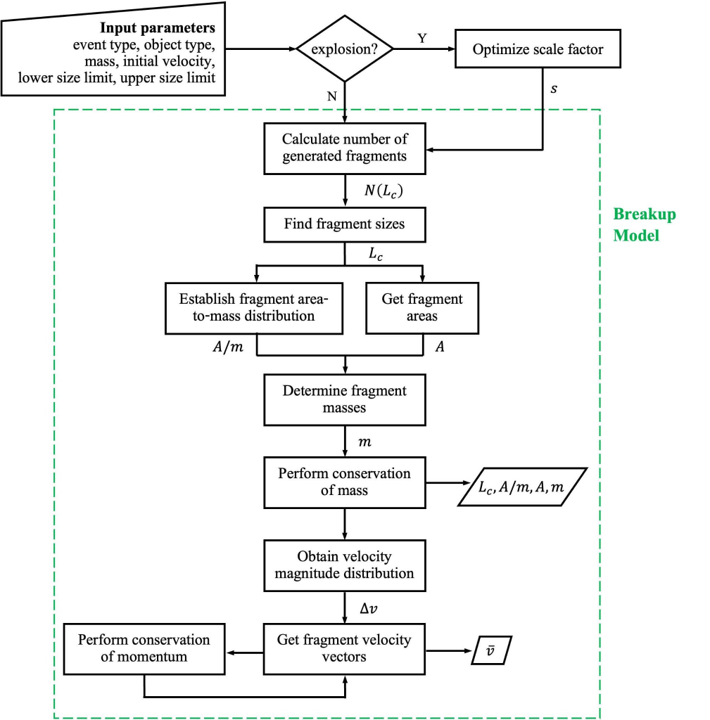
\includegraphics[width=0.75\linewidth]{NSBM_Ariel.png}
    \caption{Flowchart of NASA's Breakup Model Architecture, illustrating the sequential process for debris generation, including mass and momentum conservation. Black, Ariel. School of Aeronautics and Astronautics, Purdue University.}
    \label{fig:NBSM}
\end{figure}

\section{Traditional Propagation Methods}
Multibody orbit propagation is essential for analyzing the trajectories of both intact satellites and fragments resulting from fragmentation events. Traditional methods often focus on larger debris objects, neglecting the significant contribution of smaller fragments to collision probabilities. One of the most widely used traditional techniques for propagating two-body orbits is \textit{Cowell’s method}, which directly integrates the equations of motion by summing all gravitational and non-gravitational forces acting on the object. This method treats the object’s acceleration as a vector derived from the central body attraction and perturbing forces, such as atmospheric drag, solar radiation pressure (SRP), and third-body effects. The integration is typically performed using standard numerical schemes like Runge-Kutta or multistep methods. While Cowell’s approach is straightforward and flexible, it is also sensitive to numerical errors, especially in long-term simulations, due to the accumulation of truncation and round-off errors.

Cowell’s method integrates Newton’s second law directly:

\begin{equation}
\ddot{\mathbf{r}} = \mathbf{a}_{\text{grav}} + \sum_{i} \mathbf{a}_{i}
\end{equation}

Where:

\begin{itemize}
    \item $\mathbf{r}$ is the position vector of the satellite,
    \item $\mathbf{a}_{\text{grav}}$ is the central body gravitational acceleration,
    \begin{equation}
        \mathbf{a}_{\text{grav}} = -\frac{\mu}{r^3} \mathbf{r}
    \end{equation}
    \item $\mathbf{a}_{i}$ represents all perturbative accelerations (e.g., atmospheric drag, solar radiation pressure, third-body effects, etc.).
\end{itemize}

An alternative to Cowell’s formulation for propagating Keplerian orbits is \textit{Encke’s method}, which focuses on integrating the deviation of a perturbed orbit from a known reference orbit. Instead of computing the full trajectory from scratch, Encke’s method calculates the difference between the real orbit and the osculating elements of the reference trajectory. This differential approach improves numerical stability, particularly when dealing with small perturbations. It also allows for more efficient integration, as the main gravitational influence is analytically accounted for in the reference solution, reducing the computational load of recalculating dominant forces at every step.

Encke’s method integrates the deviation $\boldsymbol{\rho}=\mathbf{r}-\mathbf{r_0}$ from a reference orbit $\mathbf{r_0(t)}$:

\begin{equation}
\ddot{\boldsymbol{\rho}} = \mathbf{a}(\mathbf{r}_0 + \boldsymbol{\rho}) - \mathbf{a}_0(\mathbf{r}_0) - \ddot{\mathbf{r}}_0
\end{equation}

Where

\begin{itemize}
    \item $\boldsymbol{\rho}$ is the deviation vector.
    \item $\mathbf{a}(\mathbf{r}_0 + \boldsymbol{\rho})$ is the total acceleration at the true position,
    \item $\mathbf{a}_0(\mathbf{r}_0)$ is the nominal central force,
    \item $\ddot{\mathbf{r}}_0$ is the acceleration of the reference orbit.
\end{itemize}

Another classical technique is the method of variation of parameters, also known as \textit{Gauss’ method}. This method reformulates the problem in terms of time-varying orbital elements, rather than Cartesian position and velocity vectors. By applying Gauss’ planetary equations, the evolution of orbital parameters due to perturbations can be directly computed. This approach offers valuable insights into the physical mechanisms driving orbital changes, such as secular drifts or periodic variations. It is particularly useful for analyzing the long-term effects of specific perturbing forces, though it may be less suitable for orbits undergoing frequent or abrupt changes.\cite{montenbruck_satellite_2000} 

The method uses the Gauss planetary equations to describe the time derivatives of the orbital elements $(a,e,i,\Omega,\omega,\nu)$. For instance, the time derivative of the semi-major axis $a$ under perturbing accelerations $(R,T,N)$ in the radial, transverse, and normal directions is:

\begin{equation}
\frac{da}{dt} = \frac{2}{n \sqrt{1 - e^2}} \left[ e R \sin \nu + \frac{p}{r} T \right]
\end{equation}

Where:

\begin{itemize}
    \item $n$ is the mean motion,
    \item $p=a(1-e^2)$ is the semi-latus rectum,
    \item $\nu$ is the true anomaly
\end{itemize}

In contrast to the traditional propagation methods discussed in this section, symplectic integrators have been adopted in celestial mechanics due to their structure-preserving properties, particularly for Hamiltonian systems governed by conservative forces. Their ability to conserve phase-space volume and exhibit bounded energy error over long periods makes them ideal for multibody dynamics and high precision orbit propagation\cite{hubaux_symplectic_2012}.


\section{Symplectic Propagation Methods}
This research seeks to advance the modeling of orbital debris evolution by investigating the long-term behavior of fragmented spacecraft populations under the influence of multibody gravitational dynamics and non-conservative forces. The main objective is to develop and extend the applicability of symplectic orbit propagators to environments such as LEO, where dissipative forces—primarily atmospheric drag and SRP play a significant role.

While symplectic integrators are well-established in preserving energy and phase-space structure in conservative systems, their use in space applied missions and scenarios involving energy dissipation remains an open area of research. By integrating fragmentation models with N-body symplectic propagation methods, this study aims to construct a computational framework capable of simulating the forward and backward evolution of debris fields, assessing collision risk, and analyzing population growth over decades to centuries.

This work explores how these methods can improve the prediction accuracy and computational efficiency in modeling debris evolution, and quantify the impact of long-term debris propagation on the stability and sustainability of orbital environments, particularly with conservative and non-conservative forces. Ultimately, the research contributes to improve debris risk forecasting and provides insight for space traffic management and sustainability policy development.

\subsection{Overview of Symplectic Methods Applied to Orbital Mechanics}

This research develops a semi-symplectic integration approach that enables the long-term propagation of objects (active and non-active) in low Earth orbit, accounting for both conservative and non-conservative forces. The method splits the forces acting on the spacecraft into two distinct types: a Hamiltonian (conservative) gravitational component and a perturbative component that includes atmospheric drag and SRP. The framework is based on second-order symplectic splitting techniques with Extended Phase Space/Splitting Methods such as Lie-Trotter or Strang splitting, ensuring accuracy and numerical stability over long propagation times\cite{luo_applying_2017}. In general, the motion is governed by the second-order ordinary differential equation:

\begin{equation}
    \frac{d\bm{v}}{dt} = \bm{a}_{\text{grav}} + \bm{a}_{\text{drag}} + \bm{a}_{\text{SRP}}
\end{equation}

where $\bm{v}$ is the velocity vector, and the terms on the right-hand side represent the respective accelerations due to gravity, atmospheric drag, and SRP.

The gravitational acceleration is modeled as:
\begin{equation}
    \bm{a}_{\text{grav}} = -\frac{\mu}{r^3} \bm{r}
\end{equation}

Atmospheric drag is treated as a non-conservative force, defined by:

\begin{equation}
    \bm{a}_{\text{drag}} = -\frac{1}{2} \frac{C_D A}{m} \rho(v) \, v \, \bm{v}
\end{equation}
where:
\begin{itemize}
    \item $C_D$ is the drag coefficient,
    \item $A$ is the cross-sectional area,
    \item $m$ is the object mass,
    \item $\rho(v)$ is the atmospheric density.
\end{itemize}

SRP, a non-conservative force, is represented by:

\begin{equation}
    \bm{a}_{\text{SRP}} = -P_{\text{SRP}} \frac{A_{\text{SRP}}}{m} (1 + q) \, \hat{\bm{r}}_{\text{sun}}
\end{equation}
where:
\begin{itemize}
    \item $P_{\text{SRP}}$ is the solar radiation pressure,
    \item $A_{\text{SRP}}$ is the effective SRP area,
    \item $q$ is the reflectivity coefficient,
    \item $\hat{\bm{r}}_{\text{sun}}$ is the unit vector from the satellite to the Sun.
\end{itemize}

\subsection{Lie–Trotter and Strang splitting formulations}

The integration of orbital dynamics influenced by both conservative and non-conservative forces can be approached using operator splitting techniques. In this context, the total evolution operator $\Phi(\Delta t)$ is decomposed into two components: $\Phi_G$, which represents the exact or numerically accurate flow of the gravity-only system (e.g., solved via symplectic leapfrog or Kepler solver), and $\Phi_P$, which accounts for perturbative forces such as atmospheric drag and solar radiation pressure. The Lie–Trotter splitting scheme applies the perturbation and gravitational flows sequentially as $\Phi_P(\Delta t) \circ \Phi_G(\Delta t)$, while the more accurate second-order Strang splitting applies the perturbative flow in symmetric half-steps:

\begin{equation}
    \Phi(\Delta t) \approx \Phi_P\left(\frac{\Delta t}{2}\right) \circ \Phi_G(\Delta t) \circ \Phi_P\left(\frac{\Delta t}{2}\right)
\end{equation}

Figure~\ref{fig:strang_splitting_flow} shows a graphical representation of this framework, where the perturbation flow $\Phi_P$ is not integrated via a symplectic method, but instead it is applied as a direct correction to the satellite's velocity vector. The perturbation step updates the velocity according to:

\begin{equation}
    \bm{v} \leftarrow \bm{v} + \Delta t \cdot \left( \bm{a}_{\text{drag}} + \bm{a}_{\text{SRP}} \right)
\end{equation}

\begin{figure}[!htb]
    \centering
    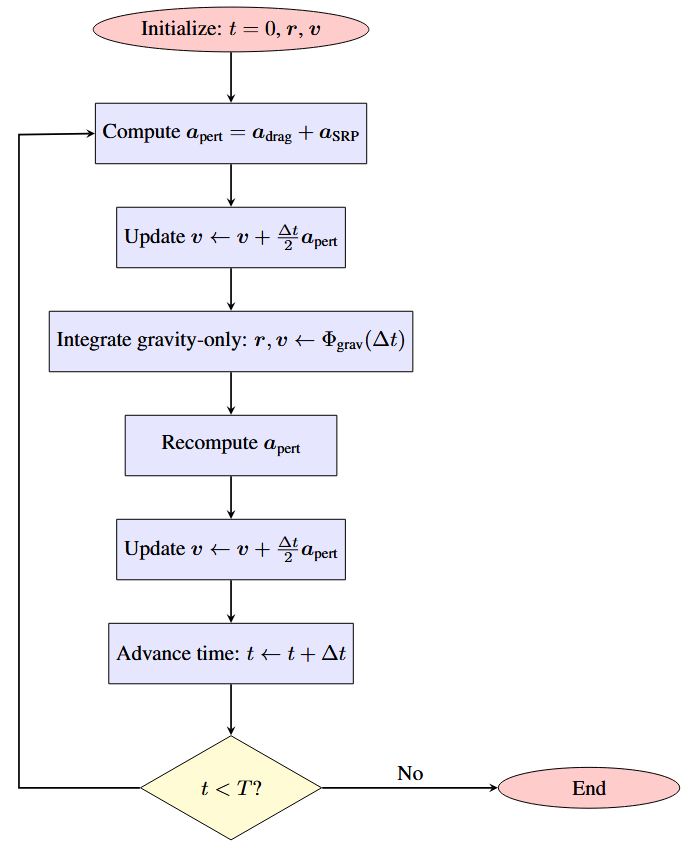
\includegraphics[width=0.6\linewidth]{Flowchart_splitting.png} 
    \caption{Flow diagram for a Strang splitting integrator, combining symplectic gravity propagation with explicit drag and solar radiation pressure perturbation steps.}
    \label{fig:strang_splitting_flow}
\end{figure}

This update ensures that the dissipative influences are incorporated while the primary symplectic structure is preserved during the gravitational flow step. As shown in Figure~\ref{fig:strang_splitting_flow}, the integration loop alternates conservative and perturbative updates symmetrically.

This hybrid approach allows for physically consistent long-term integration, maintaining energy behavior under gravity while incorporating dissipative effects without disrupting the underlying phase space structure of the Hamiltonian flow. The methodology is validated through numerical experiments of satellites in LEO and lunar transfer orbits, with comparisons against traditional Runge-Kutta integration for decay and energy drift.

\subsection*{Challenges and limitations}

Symplectic integrators are inherently designed to preserve the structure of conservative systems, particularly the Hamiltonian flow, phase space volume, and long-term energy behavior. However, drag and SRP violate these assumptions by introducing dissipative or non-Hamiltonian components into the system dynamics.

One of the primary challenges lies in the incompatibility between the symplectic framework and the nature of dissipative forces. Atmospheric drag causes continuous energy loss and angular momentum, fundamentally altering the system's phase space trajectory. SRP, while not necessarily dissipative, introduces time-dependent forcing that further deviates from canonical symplectic form.

\section{Framework Validation and Results}
To validate the accuracy, computational performance, and long-term stability of the symplectic N-body framework, simulations were conducted and benchmarked against NASA's General Mission Analysis Tool (GMAT), a high-fidelity, industry-standard orbit propagation tool.

\subsection{Case Study: Large-Scale LEO Debris Simulation}
To validate the framework's performance under a high-density N-body scenario, a simulation was conducted using a procedurally generated population of up to 20,000 spacecraft and debris objects. This approach tests the scalability and stability of the integrator when handling a large, complex population, which is representative of future debris environments.

\begin{itemize}
    \item \textbf{Population Model:} The 20,000 objects were generated with randomized but physically plausible LEO elements, as described in the propagation code. This includes altitudes from 400 to 1,000 km, eccentricities from 0 to 0.05, and inclinations from 0 to 100 degrees.
    \item \textbf{Propagation:} The full N-body simulation was propagated for a duration of 1 day (24 hours) using the \texttt{WHFast} symplectic integrator.
    \item \textbf{Force Model:} The \texttt{REBOUNDx} extension was used to incorporate non-conservative forces, including a geopotential model (J2 and J4).
    \item \textbf{Benchmark:} For accuracy validation, a representative subset of fragments was propagated in NASA's General Mission Analysis Tool (GMAT) using an identical force model for a one-to-one comparison.
\end{itemize}

\subsection{Positional Accuracy}
\begin{figure}[!htb]
    \centering
    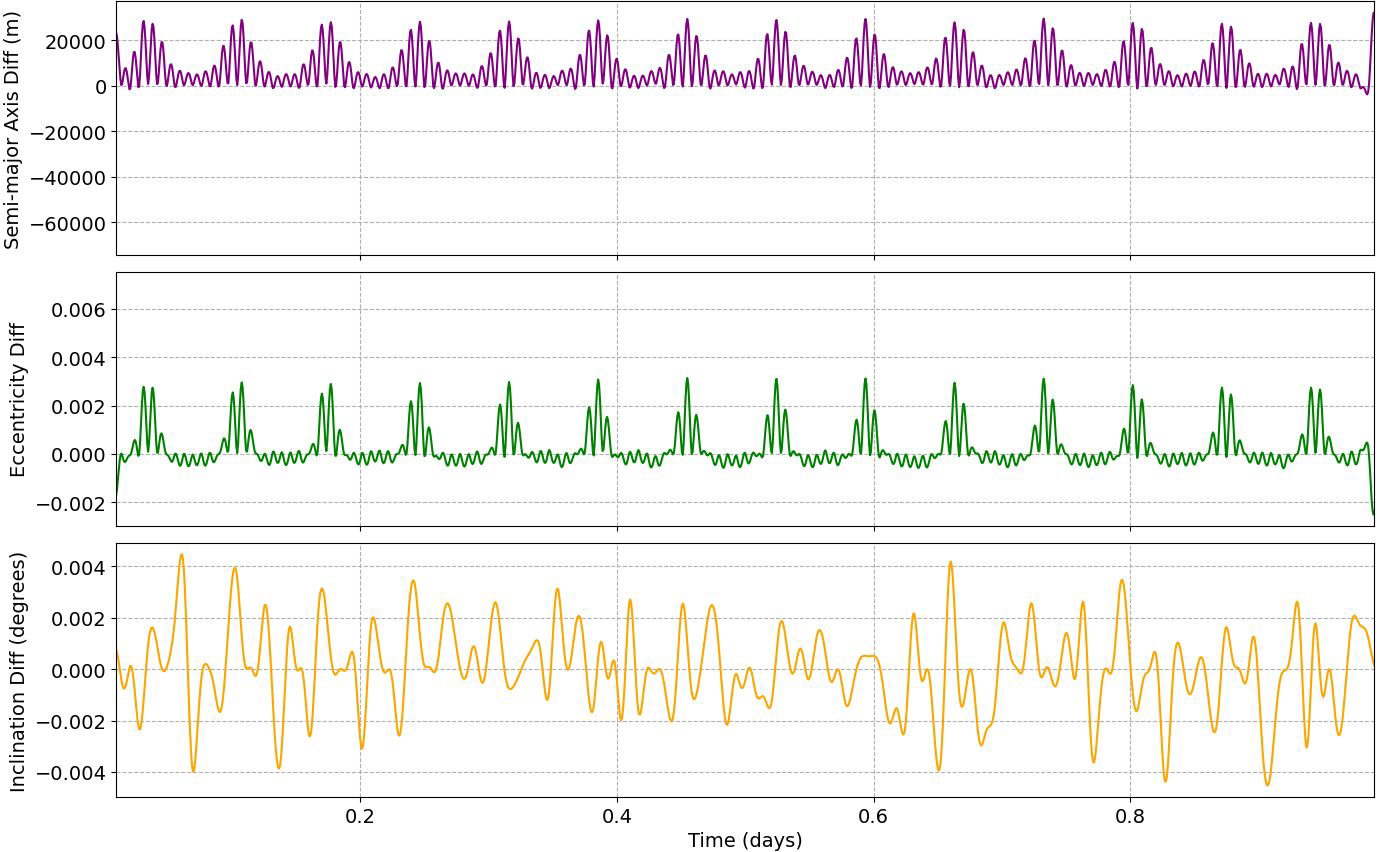
\includegraphics[width=0.95\linewidth]{element_difference.png} 
    \caption{Orbital element difference (GMAT - Symplectic) for an eccentric LEO case over a 24-hour propagation.}
    \label{fig:pos_accuracy}
\end{figure}

The primary validation metric was the consistency of the orbital elements propagated by the orbital framework against GMAT. Figure~\ref{fig:pos_accuracy} shows the difference in semi-major axis, eccentricity, and inclination for a representative fragment over a 24-hour propagation.

The results demonstrate that the orbital elements remain well-bounded. The semi-major axis difference shows a periodic variation between approximately +20,000 m and -60,000 m, while the eccentricity difference remains bounded within $\pm 0.004$ and the inclination difference within $\pm 0.004$ degrees. This confirms that the proposed framework, while exhibiting different numerical behavior, accurately captures the orbital dynamics in a way that is stable and consistent with the high-fidelity benchmark.

\subsection{Computational Scalability}
A key objective of this framework is to assess its computational scalability for large N-body populations. To quantify this, the C-based REBOUND simulation was executed multiple times, holding the propagation duration constant at 1 day while varying the number of objects (N) from 50 to 20,000. This test is designed to measure the raw performance and scalability of the symplectic N-body approach, which is a critical factor for analyzing massive debris clouds.

\begin{figure}[!htb]
    \centering
    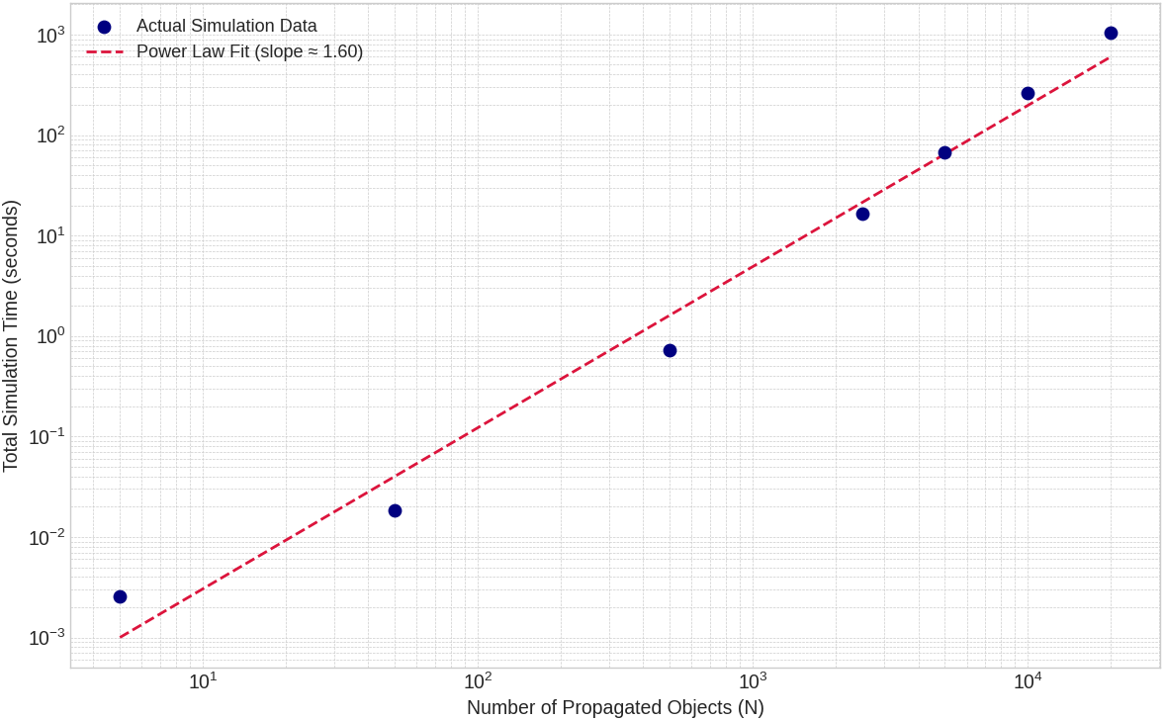
\includegraphics[width=0.95\linewidth]{scalability_plot.png}
    \caption{Total simulation time in seconds as a function of the number of propagated objects (N). The data (blue dots) fit a power law (red dashed line) with a slope of 1.60, demonstrating excellent computational scalability.}
    \label{fig:scalability_plot}
\end{figure}

The total CPU execution time for each 1-day simulation was recorded. Figure~\ref{fig:scalability_plot} plots the total simulation time as a function of the number of propagated objects. The data shows a clear power-law relationship with a slope of approximately 1.60. This demonstrates excellent, predictable scalability and proves the framework's computational feasibility for analyzing the short-term evolution of massive debris clouds. This N-body approach is profoundly more efficient than propagating each object individually in a traditional mission analysis tool.

\subsection{Long-Term Stability}
The final validation highlights the core advantage of a symplectic integrator for long-term analysis. While a direct energy-drift comparison was not performed, the long-term stability is demonstrated by comparing the orbital element evolution against GMAT.

\begin{figure}[!htb]
    \centering
    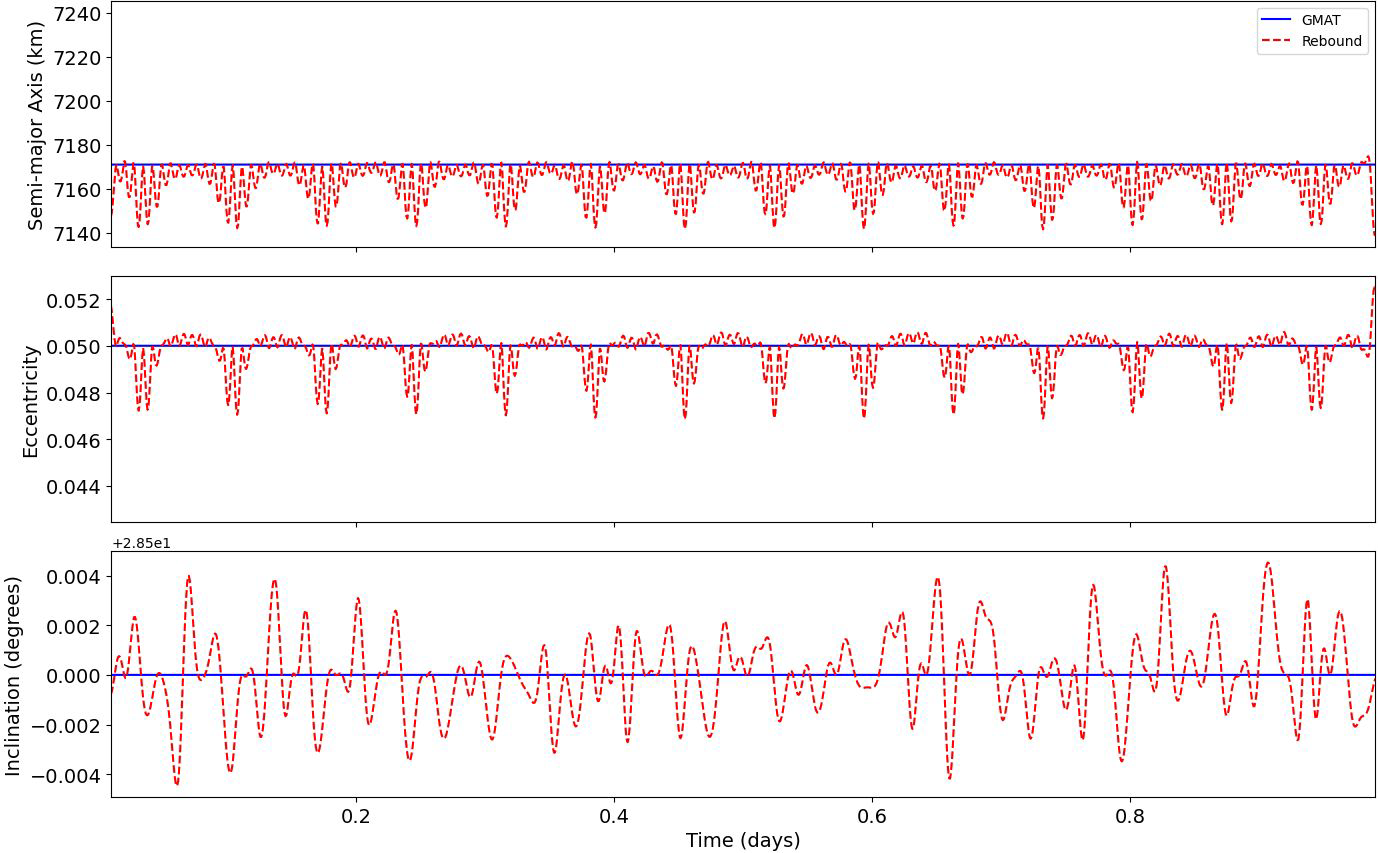
\includegraphics[width=0.95\linewidth]{element_evolution.png}
    \caption{Orbital element evolution (GMAT vs. Symplectic) over a 1-day propagation, demonstrating the bounded, non-drifting, and stable behavior of the symplectic integrator.}
    \label{fig:stability_plot}
\end{figure}

As shown in Figure~\ref{fig:stability_plot}, the orbital elements (semi-major axis, eccentricity, and inclination) from the REBOUND simulation (dashed red line) show bounded, periodic oscillations that closely match the high-fidelity GMAT propagation (solid blue line). This lack of secular (one-directional) drift in the elements proves the stability and reliability of the symplectic method for the long-term propagation required for debris evolution studies.

\section{Concluding Remarks}

A major contribution of this study was the validation of a symplectic N-body framework for
large-scale debris propagation. The methodology was benchmarked against high-fidelity tools like
GMAT, confirming the framework's ability to produce consistent orbital element evolution while
incorporating geopotential perturbations (J2 and J4).

The framework was validated against a large-scale, 20,000-object LEO simulation, demonstrating its robustness. Furthermore, the study proved the computational scalability of the N-body approach, which scales predictably with a power law of 1.6. This research leveraged the REBOUND N-body simulation framework, providing a robust, scalable, and physically-consistent tool for the astrodynamics community to analyze debris cloud evolution. Future work will focus on integrating non-conservative forces, such as atmospheric drag and solar radiation pressure, using the operator splitting methods described in this paper.

\bibliographystyle{AAS_publication}
\bibliography{articles_AIAA_ASC}

\end{document}